\documentclass[landscape]{article}

\usepackage[margin=10mm]{geometry} % Document margins
\usepackage{fontspec}
\usepackage{multicol}
\usepackage{enumitem}
\usepackage[usenames]{xcolor}
\usepackage{titlesec}

\newlist{myitemize}{itemize}{1}
\setlist[myitemize]{label=\textbullet,labelindent=-.1in,leftmargin=0pt,itemsep=0pt}

\setmainfont[Ligatures=TeX]{Linux Libertine O}
\setsansfont[Ligatures=TeX]{Linux Biolinum O}
\setmonofont[Scale=MatchLowercase]{DejaVu Sans Mono}

\titlespacing*{\subsection}{0pt}{*2}{*1.5}

\newcommand*{\prog}{\texttt}
\newcommand*{\proge}[1]{\textcolor{gray}{\textit{\# #1}}}
\setlength{\columnsep}{2\columnsep}

\begin{document}
\pagestyle{empty}

\textsf{ {\LARGE Git handout} -- Tomi Peltola, Henri Seijo, Arno Solin -- last update December 19th 2012}
\vspace{\baselineskip}\\
\begin{tabular*}{1\textwidth}{@{\extracolsep{\fill}} p{0.33\textwidth} p{0.66\textwidth}}
\begin{minipage}[t]{0.315\textwidth}
\textit{``Git is a free and open source distributed version control system designed to handle everything from small to very large projects with speed and efficiency.''} -- git-scm.com

\section{Terminology}
\begin{myitemize}
  \item \textbf{repository} (repo): a database holding different versions (history) of files under version control
  \item \textbf{working directory}: holds files, which are worked on
  \item \textbf{commit}: a snapshot of the files under version control
  \item \textbf{to commit}: to save a snapshot of the current state of files to the repository
  \item \textbf{stage} (index): composing area for commits; committing records the modifications in stage to a commit
  \item \textbf{to stage}: to add modified files from working directory to stage
  \item \textbf{branch}: named lineage of commits; multiple branches allow for isolated, parallel lines of development
  \item \textbf{to branch}: to diverge a new branch from a parent branch
  \item \textbf{conflict}: overlapping modifications in parallel branches
  \item \textbf{merge}: a commit, which handles possible conflicts between branches and joins the branches
  \item \textbf{to merge}: to bring the contents of another branch into the current branch
  \item \textbf{fast-forward merge}: merging of branches, where the merged branch is a linear continuation of the parent branch; commits in the merged branch are included in the parent branch as such
  \item \textbf{remote repository}: a copy of the repository, which can be accessed over network or filesystem
  \item \textbf{to clone}: make an independent copy of a repository
  \item \textbf{to push}: to sync repos by sending commits from the local repo to a remote repo
  \item \textbf{to pull}: to sync repos by getting commits from a remote repo
  \item \textbf{tag}: a nickname usually for a commit, e.g.\ v3.4.2
  \item \textbf{bare repository}: a repository without working files
  \end{myitemize}
\end{minipage}
&
\begin{minipage}[t]{0.6\textwidth}
  \section{Anatomy of Git repository}
  \vspace{-10mm}
  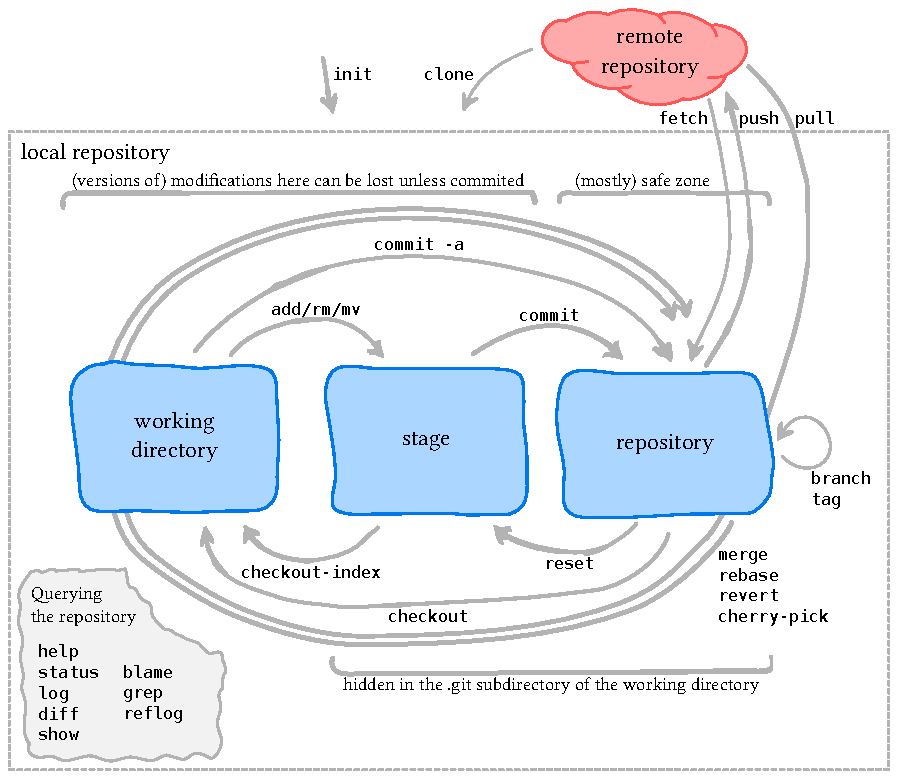
\includegraphics[scale=1.1]{gitflow} 
  \section{Merging strategies}
  \vspace{-5mm}
  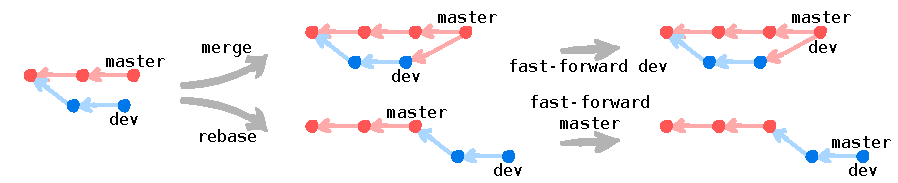
\includegraphics[scale=1.1]{merging} 
\end{minipage}
\end{tabular*}

\pagebreak
\begin{multicols*}{3}
  \section{Usage reference}

  All commands should be prefixed with \prog{git}, e.g., \prog{git help}.
  \begin{myitemize}
    \item \textbf{help}\\
      \prog{help} \proge{lists common commands}\\
      \prog{help config} \proge{help on a particular command (here \prog{config})}
  \end{myitemize}

  \subsection{Configuration}
  \begin{myitemize}
    \item \textbf{set name and email}\\
      \prog{config --global user.name Jane Smith}\\
      \prog{config --global user.email jane.smith@aalto.fi}
    \item \textbf{set editor and coloring of output}\\
      \prog{config --global core.editor nano} \proge{or vim, emacs etc.}
      \prog{config --global color.ui true}
      \vspace{\parsep}\\
      Without \prog{--global} option the commands affect only the repository in the current directory.
  \end{myitemize}

  \subsection{Creating or getting a repository}
  \begin{myitemize}
    \item \textbf{create a new repository to current directory}\\
      \prog{init}
      \vspace{\parsep}\\
      Add \prog{--shared} option to create a repository, which handles read and write permissions for unix group.
    \item \textbf{clone an existing repository}\\
      \prog{clone /local/path/repo.git} \proge{clones to repo subdir.}\\
      \prog{clone https://github.com/JuliaLang/julia.git jul} \proge{use jul subdirectory instead of julia}
      \vspace{\parsep}\\
      Add \prog{--bare} option after \prog{init} or \prog{clone} to create a bare repository. Note: \prog{--shared} with \prog{clone} is not the same option as with \prog{init}. 
  \end{myitemize}

  \subsection{Querying information}

  \begin{myitemize}
    \item \textbf{current status of repository}\\
      \prog{status}
    \item \textbf{log}\\
      \prog{log}\\
      \prog{log --oneline --graph} \proge{brief version showing branching}\\
      \prog{log --name-status} \proge{show which files changed}
    \item \textbf{differences between versions of files}\\
      \prog{diff} \proge{between working directory and stage}\\
      \prog{diff --staged} \proge{between stage and the latest commit}\\
      \prog{diff --color-words} \proge{show diff of words instead of lines}\\
      \prog{diff 11c38af a68db70 -- readme.txt} \proge{between the listed commits, only in readme.txt}
    \item \textbf{who changed and when the lines of a file}\\
      \prog{blame readme.txt}
    \item \textbf{show the message and changes of a commit}\\
      \prog{show 6dbe052}
  \end{myitemize}

  \subsection{Basic workflow}
  \begin{myitemize}
    \item \textbf{stage files and modifications}\\
      \prog{add .} \proge{stage all files in the directory}\\
      \prog{add readme.txt} \proge{listing multiple files works also}\\
      \prog{add -p readme.txt} \proge{interactively select which modifications are staged; -p works also with many other commands}\\
      \prog{rm readme.txt} \proge{removal; removes the file from filesystem}\\
      \prog{mv readme.txt readme.md} \proge{rename}
    \item \textbf{unstage}\\
      \prog{reset readme.txt}
    \item \textbf{commit}\\
      \prog{commit} \proge{commit the staged modifications}\\
      \prog{commit -m "My commit message"}\\
      \prog{commit -a} \proge{commit modifications in all tracked files (skips staging)}
    \item \textbf{get an older version of a file}\\
      \prog{checkout 6dac6bf -- readme.txt} \proge{take from 6dac6bf}
    \item \textbf{revert a commit}\\
      \prog{revert 47410c4} \proge{makes a new commit reverting 47410c4}
    \item \textbf{get files from stage to working directory}\\
      \prog{checkout-index readme.txt}
    \item \textbf{apply the changes in a commit}\\
      \prog{cherry-pick 7360d6a} \proge{makes a new commit with the changes in 7360d6a}
    \item \textbf{tag}\\
      \prog{tag v1.0} \proge{name the latest commit v1.0}
  \end{myitemize}

  \subsection{Branching and merging}

  \begin{myitemize}
    \item \textbf{list, create and delete branches}\\
      \prog{branch -a} \proge{list}\\
      \prog{branch dev} \proge{diverge a new branch with name dev}\\
      \prog{checkout -b dev} \proge{create a new branch and change to it}\\
      \prog{checkout -b dev origin/dev} \proge{create a local branch from a fetched remote branch (see below)}\\
      \prog{branch -d dev} \proge{delete}
    \item \textbf{change to a branch}\\
      \prog{checkout dev} \proge{change to branch dev}
    \item \textbf{merge branches}\\
      \prog{merge dev} \proge{merges dev branch to current branch}
      \vspace{\parsep}\\
      Note: branch name is a reference to the latest commit in the branch. \prog{HEAD} is a reference to the latest commit in the current branch. \prog{FETCH\_HEAD} is a reference to the latest commit in a fetched remote branch (see below).
  \end{myitemize}

  \subsection{Synchronizing with remote repositories}

  \begin{myitemize}
    \item \textbf{list, add and remove remotes}\\
      \prog{remote -v} \proge{list remotes}\\
      \prog{remote add becs\\\hspace*{5mm}ssh://jsmith@url.aalto.fi/path/to/repo.git}\\\proge{add with name becs; use ssh with username jsmith}\\
      \prog{remote rm becs} \proge{remove}
    \item \textbf{fetch changes from a remote}\\
      \prog{fetch becs master} \proge{fetch master branch from becs; do not merge the changes}
    \item \textbf{pull changes from a remote}\\
      \prog{pull becs master} \proge{tries to also merge the changes}
    \item \textbf{push changes to a remote}\\
      \prog{push becs master} \proge{pushes master branch}
      \vspace{\parsep}\\
      Note: remote \prog{origin} is automatically added on clone.
  \end{myitemize}

  \subsection{Rewriting history}

  Never rewrite shared history!
  \begin{myitemize}
    \item \textbf{amend a previous commit or change its message}\\
      \prog{commit --amend} \proge{after, e.g., adding a forgotten file to stage}
    \item \textbf{rebase a branch to include the progress in a parent branch}\\
      \prog{rebase master} \proge{assuming master is the parent branch}
    \item \textbf{combine, remove and edit commits}\\
      \prog{rebase -i fe18b87} \proge{prompt for commits after fe18b87}
  \end{myitemize}

  \section{Resources}

  \begin{myitemize}
  \item \textbf{Git homepage}: git-scm.com
  \item \textbf{Pro Git book}: git-scm.com/book
  \item \textbf{Stackoverflow}: stackoverflow.com/questions/tagged/git
  \item \textbf{GitHub}: github.com -- popular Git hosting on web
  \item \textbf{Bitbucket}: bitbucket.org -- popular Git hosting on web
  \end{myitemize}

\end{multicols*}
\end{document}
